\documentclass[11pt]{article}
\usepackage[myheadings]{fullpage}
\usepackage{fancyhdr}
\usepackage{lastpage}
\usepackage{graphicx, wrapfig, subcaption, setspace, booktabs}
\usepackage[font=small, labelfont=bf]{caption}
\usepackage{fourier}
\usepackage[protrusion=true, expansion=true]{microtype}
\usepackage[english]{babel}
\usepackage[final]{hyperref} 
\usepackage{url, lipsum}
\usepackage{float}
\usepackage{amsmath}
\usepackage{mathpazo}
\usepackage{mathtools}
\usepackage{multicol}
\usepackage[none]{hyphenat}
\usepackage{siunitx}
\usepackage[RPvoltages]{circuitikz}
\usepackage{gensymb}
\usepackage[framed,numbered]{matlab-prettifier}
\usepackage{chngcntr}
\usepackage[T1]{fontenc}
\usepackage{listings}
\usepackage{tabularx}
\usepackage{adjustbox}


\newcommand{\HRule}[1]{\rule{\linewidth}{#1}}
\newcommand*\mean[1]{\overline{#1}}
\onehalfspacing
\setcounter{tocdepth}{5}
\setcounter{secnumdepth}{5}

\lstdefinestyle{sql}{
    language=SQL,
    basicstyle=\small\ttfamily,
    keywordstyle=\color{blue}\bfseries,
    commentstyle=\color{gray},
    stringstyle=\color{red},
    numbers=left,
    numberstyle=\tiny\color{gray},
    stepnumber=1,
    numbersep=5pt,
    backgroundcolor=\color{white},
    showspaces=false,
    showstringspaces=false,
    showtabs=false,
    frame=single,
    tabsize=4,
    captionpos=b,
    breaklines=true,
    breakatwhitespace=false,
    escapeinside={\%*}{*)},
    morekeywords={SELECT, FROM, WHERE, ORDER BY, GROUP BY, JOIN, ON, INSERT INTO, VALUES, UPDATE, SET, DELETE FROM}
}




%-------------------------------------------------------------------------------
% HEADER & FOOTER
%-------------------------------------------------------------------------------
\pagestyle{fancy}
\fancyhf{}
\setlength\headheight{15pt}
\fancyhead[L]{CSCI403: Database Management}
\fancyhead[R]{Ching}
\fancyfoot[R]{Page \thepage\ of \pageref{LastPage}}
%-------------------------------------------------------------------------------
% TITLE PAGE
%-------------------------------------------------------------------------------
\title{\uppercase{Enhancing Data Analysis and Scoring Systems for the Solar Car Challenge Foundation: A Comprehensive Analysis of Real-World Data}}
\author{Brandon Ching}



\begin{document}
\makeatletter
\begin{titlepage}
    \begin{center}
        \normalsize
        \vspace*{2.5cm}
        \LARGE\textbf{CSCI403: Database Management \bigbreak
            \@title}
        \normalsize
        \\ [3.5cm]
        submitted to\\
        \textbf{
        Christopher Painter-Wakefield\\
        Colorado School of Mines
        \\ [1cm]
        \@date
        \\ [4cm]
        By\\
        \@author}
    \end{center}
\end{titlepage}
\makeatother

%-------------------------------------------------------------------------------
% BODY
%-------------------------------------------------------------------------------
\section{Background and Overview}

The aim of this project and subsequent report is to analyze a real-world dataset using the principles and techniques learned in the CSCI403 Database Management course. Specifically, the dataset under scrutiny comprises event logs from the 2022 Solar Car Challenge. Utilizing SQL queries, we intend to extract and scrutinize data from this set, identifying trends, patterns, and insights that could enhance future iterations of the event. The report will encompass an overview of the dataset, details of the analysis performed, and a summary of findings.

I chose this dataset due to my involvement as a volunteer and judge in the Solar Car Challenge. Having contributed to the development of the timing and scoring system used during the event, I continue to collaborate with the organization to refine this system. The analyses conducted herein will inform and influence future events, including the upcoming 2024 edition.

\section{About the Dataset}

The dataset under examination is a proprietary collection provided by The Solar Car Challenge Foundation (SCCF). As a non-profit organization, SCCF hosts the Solar Car Challenge—an annual event where high school students from around the world design, build, and race solar vehicles. The dataset comprises event logs from the 2022 challenge, containing scoring and timing data for each participating team.

The data was extracted by retrieving CSV files exported from a PostgreSQL database post-event. These files generated two primary tables: \texttt{score\_rawclickeydata} and \texttt{score\_diary}. The former records "mark lap" events logged by the timing and scoring system, while the latter documents events noted by judges during the challenge. Both tables are linked by a common field, \texttt{team\_id}, which serves as a unique identifier for each participating team.

While the archived dataset contained additional tables detailing participating teams, judges, and event metadata, the analysis primarily focused on scoring and timing data. These supplementary tables provided contextual information but were not integral to the analysis.

\subsection{score\_rawclickeydata Table}

As shown in Table \ref{tab:score_rawclickeydata}, the \texttt{score\_rawclickeydata} table contains the following fields:

\begin{itemize}
    \item \textbf{id:} Unique identifier for each record.
    \item \textbf{day:} Integer value representing the day of the event (1-4).
    \item \textbf{team\_id:} ID of the team that the record pertains to.
    \item \textbf{time\_stamp:} UTC timestamp of the event.
    \item \textbf{judge:} Name of the judge who recorded the event.
\end{itemize}

\begin{table}[H]
    \centering
    \begin{tabular}{|c|c|c|c|c|}
        \hline
        \textbf{id} & \textbf{day} & \textbf{team\_id} & \textbf{time\_stamp}       & \textbf{judge}  \\
        \hline
        3910        & 1            & 1                 & 2022-07-17 13:03:32.454000 & lsjaye-Brandon  \\
        3912        & 1            & 1                 & 2022-07-17 13:03:32.685000 & 8hi33y-Liam     \\
        3913        & 1            & 1                 & 2022-07-17 13:03:33.269000 & 8wk342-Michael1 \\
        3914        & 1            & 1                 & 2022-07-17 13:05:43.315000 & 8wk342-Michael1 \\
        3915        & 1            & 1                 & 2022-07-17 13:05:43.294000 & c2dvxj-Ricardo  \\
        3919        & 1            & 2                 & 2022-07-17 13:05:57.428000 & c2dvxj-Ricardo  \\
        3920        & 1            & 2                 & 2022-07-17 13:05:57.446000 & lsjaye-Brandon  \\
        3921        & 1            & 2                 & 2022-07-17 13:05:57.388000 & 8wk342-Michael1 \\
        3922        & 1            & 5                 & 2022-07-17 13:08:07.675000 & lsjaye-Brandon  \\
        3923        & 1            & 5                 & 2022-07-17 13:08:07.932000 & 8hi33y-Liam     \\
        \hline
    \end{tabular}
    \caption{score\_rawclickeydata table sample data.}
    \label{tab:score_rawclickeydata}
\end{table}

\subsection{score\_diary Table}
As shown in Table \ref{tab:score_diary}, the \texttt{score\_diary} table contains the following fields:

\begin{itemize}
    \item \textbf{id:} Unique identifier for each record.
    \item \textbf{day:} Integer value representing the day of the event (1-4).
    \item \textbf{team\_id:} ID of the team that the record pertains to.
    \item \textbf{time\_stamp:} UTC timestamp of the event.
    \item \textbf{judge:} Name of the judge who recorded the event.
    \item \textbf{event:} Description of the event recorded (e.g., "mark lap", "enter track", etc).
    \item \textbf{num\_passengers:} Number of passengers in the vehicle at the time of the event.
\end{itemize}

\begin{table}[H]
    \centering
    \begin{tabular}{|c|c|c|c|c|c|}
        \hline
        \textbf{Id} & \textbf{Day} & \textbf{time\_stamp}       & \textbf{judge} & \textbf{event} & \textbf{num\_passengers} \\
        \hline
        20          & 1            & 2022-07-17 13:00:50.434000 & igwgh3-Adayr   & Enter Track    & <null>                   \\
        21          & 2            & 2022-07-17 13:01:26.072000 & igwgh3-Adayr   & Enter Track    & <null>                   \\
        22          & 5            & 2022-07-17 13:03:26.401000 & igwgh3-Aldayr  & Enter Track    & <null>                   \\
        23          & 7            & 2022-07-17 13:04:25.393000 & igwgh3-Aldayr  & Enter Track    & <null>                   \\
        24          & 8            & 2022-07-17 13:05:24.882000 & igwgh3-Aldayr  & Enter Track    & <null>                   \\
        25          & 9            & 2022-07-17 13:06:24.519000 & igwgh3-Aldayr  & Enter Track    & <null>                   \\
        26          & 10           & 2022-07-17 13:07:26.263000 & igwgh3-Aldayr  & Enter Track    & <null>                   \\
        27          & 11           & 2022-07-17 13:08:24.447000 & 6c8fwd-Lucas   & Enter Track    & <null>                   \\
        28          & 11           & 2022-07-17 13:08:45.302000 & 6c8fwd-Lucas   & Exit Track     & <null>                   \\
        29          & 12           & 2022-07-17 13:09:25.215000 & 6c8fwd-Lucas   & Enter Track    & <null>                   \\
        \hline
    \end{tabular}
    \caption{score\_diary table sample data.}
    \label{tab:score_diary}
\end{table}

\subsection{Data Collection Method}

The dataset was compiled using a custom-built timing and scoring system tailored for the Solar Car Challenge. This system features a bespoke web interface enabling judges to record team lap completions and predefined events. Typically, a minimum of three judges mark lap completions and events, resulting in at least three separate records for each valid lap.

\subsection{License and Privacy}

This dataset remains the property of SCCF and should not be shared or distributed without their explicit permission. To protect participant privacy, any personally identifiable information has been removed from the dataset.






\section{Data Analysis}

During the data analysis phase, 4 primary queries were developed to extract and analyze data from the dataset. These queries aimed to provide insights into the performance of participating teams, identify trends, and refine the scoring system. The queries were designed to calculate the total lap credit earned by each team on a given day, along with the average and best lap times for each team. Additionally, the queries determined the total laps completed by each team, accounting for penalties and bonus laps. The results were then sorted by division and day's lap credit, with the leading team in each division assigned a rank of 1. The queries also aggregated supplementary data such as team names and websites to provide context to the results.

These queries were:

\begin{enumerate}
    \item \textbf{Audit Query:} Provide a detailed data dump of the scoring and timing data. The output of this query allows for a comprehensive review of the data, ensuring the accuracy and integrity of the scoring system. This query is the backbone of the scoring system and is referenced by all following queries.
    \item \textbf{Live Scoring Query:} Process the raw data in real time, allowing for the results of the query to be displayed on a live web interface. This query provides real-time unofficial results to participants and spectators, enhancing the event experience.
    \item \textbf{Specific Team Lap Stats:} For a specific team, calculate the lap times for a specified day of the event. This query provides detailed insights into the performance of individual teams, allowing for targeted analysis and feedback. This also has the added ability to plot teams lap times over the course of the event.
    \item \textbf{Judge accuracy Query:} Analyze the data to determine the accuracy of individual judges. This query calculates the average deviation of each judge's lap times from the mean, providing insights into the consistency and reliability of each judge.
\end{enumerate}

\noindent
NOTE: Most of the queries developed for this analysis ended up being extremely long and complicated. I apologies for them being hard to read and follow.

\pagebreak
\subsection{Audit Query}
\label{sec:audit_query}

At the core of the scoring system is the audit query, which provides a detailed data dump of the scoring and timing data. This query is saved as a view as \texttt{live\_rawscore} in the database allowing the data to be easily accessed and reviewed. The audit query outputs the following fields:

\begin{itemize}
    \item \textbf{id:} A unique identifier for each record.\footnote{This field is not a key due to the fact it displays ids from both the \texttt{score\_rawclickeydata} and \texttt{score\_diary} tables. Each of these tables had their own unique id auto incrementing field. This results in some overlapping ids. This issue has since been resolved in the current version of the database that will be used for 2024.}
    \item \textbf{day:} Integer value representing the day of the event (1-4).
    \item \textbf{team\_id:} ID of the team that the record pertains to.
    \item \textbf{time\_stamp:} UTC timestamp of the event.
    \item \textbf{judge:} Name of the judge who recorded the event.
    \item \textbf{event:} Description of the event recorded (e.g., "mark lap", "enter track", etc)
    \item \textbf{num\_passengers:} Number of passengers in the vehicle at the time of the event.
    \item \textbf{passengers\_change\_timestamp:} Timestamp of the last change of passengers.
    \item \textbf{any\_event\_prev\_time\_diff:} Time difference between the current event and the previous event.
    \item \textbf{any\_event\_next\_time\_diff:} Time difference between the current event and the next event.
    \item \textbf{same\_event\_prev\_time\_stamp:} Timestamp of the previous event of the same type.
    \item \textbf{same\_event\_prev\_time\_diff:} Time difference between the current event and the previous event of the same type.
    \item \textbf{same\_event\_prev\_2\_time\_diff:} Time difference between the current event and the event before the previous event of the same type.
    \item \textbf{same\_event\_next\_time\_stamp:} Timestamp of the next event of the same type.
    \item \textbf{same\_event\_next\_time\_diff:} Time difference between the current event and the next event of the same type.
    \item \textbf{same\_event\_next\_2\_time\_diff:} Time difference between the current event and the event after the next event of the same type.
    \item \textbf{same\_event\_same\_judge\_next\_time\_diff:} Time difference between the current event and the next event of the same type recorded by the same judge.
    \item \textbf{last\_time\_entered\_track:} Timestamp of the last time the team entered the track.
    \item \textbf{last\_time\_exited\_track:} Timestamp of the last time the team exited the track.
    \item \textbf{current\_location:} Description of the current location of the team (e.g., "on track" or "off track").
    \item \textbf{confirmed\_lap:} Boolean value indicating whether the lap was confirmed.
    \item \textbf{lap\_click\_count:} Number of times the lap was clicked.
    \item \textbf{lap\_click\_any:} Boolean value indicating whether the lap was clicked at all.
    \item \textbf{self\_confirmed\_lap:} Boolean value indicating whether the lap was self-confirmed.
    \item \textbf{num\_passengers\_impute:} Number of passengers imputed by the system.
    \item \textbf{lap\_time:} Time taken to complete the lap.
    \item \textbf{low\_confidence\_lap:} Description of the confidence level of the lap.
\end{itemize}

Due to the number of fields and the complexity of the query, a sample of the query results is not provided in this report. However, the full query is included in Listing \ref{lst:sql_audit_query}.


\begin{lstlisting}[style=sql, caption={Full Audit query}, label={lst:sql_audit_query}]
SELECT raw_and_diary_2.id,
    raw_and_diary_2.day,
    raw_and_diary_2.team_id,
    raw_and_diary_2.time_stamp,
    raw_and_diary_2.judge,
    raw_and_diary_2.event,
    raw_and_diary_2.num_passengers,
    raw_and_diary_2.passengers_change_timestamp,
    raw_and_diary_2.any_event_prev_time_diff,
    raw_and_diary_2.any_event_next_time_diff,
    raw_and_diary_2.same_event_prev_time_stamp,
    raw_and_diary_2.same_event_prev_time_diff,
    raw_and_diary_2.same_event_prev_2_time_diff,
    raw_and_diary_2.same_event_next_time_stamp,
    raw_and_diary_2.same_event_next_time_diff,
    raw_and_diary_2.same_event_next_2_time_diff,
    raw_and_diary_2.same_event_same_judge_next_time_diff,
    raw_and_diary_2.last_time_entered_track,
    raw_and_diary_2.last_time_exited_track,
    raw_and_diary_2.current_location,
    raw_and_diary_2.confirmed_lap,
    raw_and_diary_2.lap_click_count,
    raw_and_diary_2.lap_click_any,
    raw_and_diary_2.self_confirmed_lap,
    raw_and_diary_2.num_passengers_impute,
    CASE
      WHEN raw_and_diary_2.num_passengers_impute IS NOT NULL
        THEN
          raw_and_diary_2.num_passengers_impute *
          raw_and_diary_2.confirmed_lap
      ELSE raw_and_diary_2.confirmed_lap
      END AS lap_credit,
    CASE
      WHEN raw_and_diary_2.lap_click_any >=
           1 AND
           raw_and_diary_2.same_event_prev_time_stamp >=
           COALESCE(
               raw_and_diary_2.last_time_entered_track,
               '2021-01-01 00:00:00'::timestamp without time zone)
        THEN
          raw_and_diary_2.time_stamp -
          raw_and_diary_2.same_event_prev_time_stamp
      WHEN raw_and_diary_2.lap_click_any >=
           1 AND
           COALESCE(
               raw_and_diary_2.same_event_prev_time_stamp,
               '2021-01-01 00:00:00'::timestamp without time zone) <
           raw_and_diary_2.last_time_entered_track
        THEN
          raw_and_diary_2.time_stamp -
          raw_and_diary_2.last_time_entered_track
      ELSE '00:00:00'::interval
      END AS lap_time,
    CASE
      WHEN
          raw_and_diary_2.lap_click_count =
          1
        THEN 'single click lap'::text
      WHEN raw_and_diary_2.lap_click_count =
           2 AND
           raw_and_diary_2.self_confirmed_lap =
           1
        THEN 'self confirmed lap'::text
      WHEN raw_and_diary_2.lap_click_count >=
           2 AND
           (raw_and_diary_2.current_location <> ALL
            (ARRAY ['on track'::text, 'leaving track'::text]))
        THEN 'check car location'::text
      ELSE ''::text
      END AS low_confidence_lap
FROM (SELECT raw_and_diary_1.id,
          raw_and_diary_1.day,
          raw_and_diary_1.team_id,
          raw_and_diary_1.time_stamp,
          raw_and_diary_1.judge,
          raw_and_diary_1.event,
          raw_and_diary_1.num_passengers,
          raw_and_diary_1.passengers_change_timestamp,
          raw_and_diary_1.any_event_prev_time_diff,
          raw_and_diary_1.any_event_next_time_diff,
          raw_and_diary_1.same_event_prev_time_stamp,
          raw_and_diary_1.same_event_prev_time_diff,
          raw_and_diary_1.same_event_prev_2_time_diff,
          raw_and_diary_1.same_event_next_time_stamp,
          raw_and_diary_1.same_event_next_time_diff,
          raw_and_diary_1.same_event_next_2_time_diff,
          raw_and_diary_1.same_event_same_judge_next_time_diff,
          raw_and_diary_1.last_time_entered_track,
          raw_and_diary_1.last_time_exited_track,
          CASE
            WHEN
                raw_and_diary_1.last_time_entered_track >
                raw_and_diary_1.last_time_exited_track
              THEN 'on track'::text
            WHEN
                raw_and_diary_1.last_time_entered_track IS NOT NULL AND
                raw_and_diary_1.last_time_exited_track IS NULL
              THEN 'on track'::text
            WHEN raw_and_diary_1.last_time_entered_track <
                 raw_and_diary_1.last_time_exited_track AND
                 (raw_and_diary_1.time_stamp -
                  raw_and_diary_1.last_time_exited_track) <=
                 '00:00:05'::interval
              THEN 'leaving track'::text
            WHEN
                raw_and_diary_1.last_time_entered_track <
                raw_and_diary_1.last_time_exited_track
              THEN 'in garage'::text
            ELSE 'unknown location'::text
            END                         AS current_location,
          CASE
            WHEN lower(raw_and_diary_1.event::text) =
                 'mark lap'::text AND
                 raw_and_diary_1.same_event_next_time_diff <=
                 '00:00:30'::interval AND
                 COALESCE(
                     raw_and_diary_1.same_event_prev_time_diff,
                     '00:10:00'::interval) >=
                 '00:00:31'::interval
              THEN 1
            WHEN lower(raw_and_diary_1.event::text) =
                 'mark lap'::text AND
                 raw_and_diary_1.same_event_next_time_diff <=
                 '00:00:30'::interval AND
                 raw_and_diary_1.same_event_prev_time_diff IS NULL
              THEN 1
            ELSE 0
            END                         AS confirmed_lap,
          CASE
            WHEN lower(raw_and_diary_1.event::text) =
                 'mark lap'::text AND
                 COALESCE(
                     raw_and_diary_1.same_event_prev_time_diff,
                     '00:10:00'::interval) >=
                 '00:00:31'::interval AND
                 raw_and_diary_1.same_event_next_time_diff <=
                 '00:00:30'::interval AND
                 raw_and_diary_1.same_event_next_2_time_diff <=
                 '00:00:30'::interval
              THEN 3
            WHEN lower(raw_and_diary_1.event::text) =
                 'mark lap'::text AND
                 COALESCE(
                     raw_and_diary_1.same_event_prev_time_diff,
                     '00:10:00'::interval) >=
                 '00:00:31'::interval AND
                 raw_and_diary_1.same_event_next_time_diff <=
                 '00:00:30'::interval
              THEN 2
            WHEN lower(raw_and_diary_1.event::text) =
                 'mark lap'::text AND
                 COALESCE(
                     raw_and_diary_1.same_event_prev_time_diff,
                     '00:10:00'::interval) >=
                 '00:00:31'::interval
              THEN 1
            ELSE 0
            END                         AS lap_click_count,
          CASE
            WHEN lower(raw_and_diary_1.event::text) =
                 'mark lap'::text AND
                 COALESCE(
                     raw_and_diary_1.same_event_prev_time_diff,
                     '00:10:00'::interval) >=
                 '00:00:31'::interval
              THEN 1
            ELSE 0
            END                         AS lap_click_any,
          CASE
            WHEN lower(raw_and_diary_1.event::text) =
                 'mark lap'::text AND
                 raw_and_diary_1.same_event_same_judge_next_time_diff <=
                 '00:00:30'::interval
              THEN 1
            ELSE 0
            END                         AS self_confirmed_lap,
          num_pass_diary.num_passengers AS num_passengers_impute
   FROM (SELECT raw_and_diary.id,
                raw_and_diary.day,
                raw_and_diary.team_id,
                raw_and_diary.time_stamp,
                raw_and_diary.judge,
                raw_and_diary.event,
                raw_and_diary.num_passengers,
                max(
                CASE
                  WHEN
                      COALESCE(
                          raw_and_diary.num_passengers,
                          '-1'::integer) >
                      0
                    THEN raw_and_diary.time_stamp
                  ELSE NULL::timestamp without time zone
                  END)
                OVER (PARTITION BY raw_and_diary.team_id,
                  (EXTRACT(
                      day
                      FROM
                      raw_and_diary.time_stamp))
                  ORDER BY raw_and_diary.time_stamp,
                    raw_and_diary.id
                  ROWS UNBOUNDED PRECEDING) AS passengers_change_timestamp,
                raw_and_diary.time_stamp -
                lag(
                raw_and_diary.time_stamp,
                1)
                OVER (PARTITION BY raw_and_diary.team_id
                  ORDER BY raw_and_diary.time_stamp,
                    raw_and_diary.id)       AS any_event_prev_time_diff,
                lead(
                raw_and_diary.time_stamp,
                1)
                OVER (PARTITION BY raw_and_diary.team_id
                  ORDER BY raw_and_diary.time_stamp,
                    raw_and_diary.id) -
                raw_and_diary.time_stamp    AS any_event_next_time_diff,
                lag(
                raw_and_diary.time_stamp,
                1)
                OVER (PARTITION BY raw_and_diary.team_id,
                  raw_and_diary.event
                  ORDER BY raw_and_diary.time_stamp,
                    raw_and_diary.id)       AS same_event_prev_time_stamp,
                raw_and_diary.time_stamp -
                lag(
                raw_and_diary.time_stamp,
                1)
                OVER (PARTITION BY raw_and_diary.team_id,
                  raw_and_diary.event
                  ORDER BY raw_and_diary.time_stamp,
                    raw_and_diary.id)       AS same_event_prev_time_diff,
                raw_and_diary.time_stamp -
                lag(
                raw_and_diary.time_stamp,
                2)
                OVER (PARTITION BY raw_and_diary.team_id,
                  raw_and_diary.event
                  ORDER BY raw_and_diary.time_stamp,
                    raw_and_diary.id)       AS same_event_prev_2_time_diff,
                lead(
                raw_and_diary.time_stamp,
                1)
                OVER (PARTITION BY raw_and_diary.team_id,
                  raw_and_diary.event
                  ORDER BY raw_and_diary.time_stamp,
                    raw_and_diary.id)       AS same_event_next_time_stamp,
                lead(
                raw_and_diary.time_stamp,
                1)
                OVER (PARTITION BY raw_and_diary.team_id,
                  raw_and_diary.event
                  ORDER BY raw_and_diary.time_stamp,
                    raw_and_diary.id) -
                raw_and_diary.time_stamp    AS same_event_next_time_diff,
                lead(
                raw_and_diary.time_stamp,
                2)
                OVER (PARTITION BY raw_and_diary.team_id,
                  raw_and_diary.event
                  ORDER BY raw_and_diary.time_stamp,
                    raw_and_diary.id) -
                raw_and_diary.time_stamp    AS same_event_next_2_time_diff,
                lead(
                raw_and_diary.time_stamp,
                1)
                OVER (PARTITION BY raw_and_diary.team_id,
                  raw_and_diary.event,
                  raw_and_diary.judge
                  ORDER BY raw_and_diary.time_stamp,
                    raw_and_diary.id) -
                raw_and_diary.time_stamp    AS same_event_same_judge_next_time_diff,
                max(
                CASE
                  WHEN
                      lower(raw_and_diary.event::text) =
                      'enter track'::text
                    THEN raw_and_diary.time_stamp
                  ELSE NULL::timestamp without time zone
                  END)
                OVER (PARTITION BY raw_and_diary.team_id,
                  (EXTRACT(
                      day
                      FROM
                      raw_and_diary.time_stamp))
                  ORDER BY raw_and_diary.time_stamp,
                    raw_and_diary.id ROWS UNBOUNDED PRECEDING)
                                            AS last_time_entered_track,
                max(
                CASE
                  WHEN
                      lower(raw_and_diary.event::text) =
                      'exit track'::text
                    THEN raw_and_diary.time_stamp
                  ELSE NULL::timestamp without time zone
                  END)
                OVER (PARTITION BY raw_and_diary.team_id,
                  (EXTRACT(
                      day
                      FROM
                      raw_and_diary.time_stamp))
                  ORDER BY raw_and_diary.time_stamp,
                    raw_and_diary.id ROWS UNBOUNDED PRECEDING)
                                            AS last_time_exited_track
         FROM (SELECT score_rawclickeydata.id,
                      score_rawclickeydata.day,
                      score_rawclickeydata.team_id,
                      score_rawclickeydata.time_stamp,
                      score_rawclickeydata.judge,
                      'mark lap'::character varying AS event,
                      '-1'::integer                 AS num_passengers
               FROM score_rawclickeydata
               UNION ALL
               SELECT score_diary.id,
                      score_diary.day,
                      score_diary.team_id,
                      score_diary.time_stamp,
                      score_diary.judge,
                      score_diary.event,
                      score_diary.num_passengers
               FROM score_diary) raw_and_diary
         ORDER BY raw_and_diary.team_id,
                  raw_and_diary.time_stamp,
                  raw_and_diary.id) raw_and_diary_1
          LEFT JOIN (SELECT score_diary.time_stamp,
                            score_diary.team_id,
                            score_diary.num_passengers
                     FROM score_diary) num_pass_diary
                    ON num_pass_diary.time_stamp =
                       raw_and_diary_1.passengers_change_timestamp AND
                       raw_and_diary_1.team_id =
                       num_pass_diary.team_id
   ORDER BY raw_and_diary_1.team_id,
            raw_and_diary_1.time_stamp,
            raw_and_diary_1.id) raw_and_diary_2
ORDER BY raw_and_diary_2.team_id,
      raw_and_diary_2.time_stamp,
      raw_and_diary_2.id;
\end{lstlisting}


\pagebreak
\subsection{Live Scoring Query}

The primary objective in analyzing this dataset was to refine the precision and efficiency of the scoring system. Previously, achieving this involved labor-intensive manual review to categorize similar events and ensure each category had multiple validating records. This process was time-consuming and prone to error. The new query, as detailed in Listing \ref{lst:sql_live_scoring_query}, computes the total lap credit earned by each team on a given day, along with the average and best lap times for each team. Additionally, it determines the total laps completed by each team, accounting for penalties and bonus laps. The resulting data is then sorted by division and day's lap credit, with the leading team in each division assigned a rank of 1. The query also aggregates supplementary data such as team names and websites to provide context to the results. A sample of the query results for day 3 of the 2021 Solar Car Challenge is presented in Table \ref{tab:solar_car_data}.

The resulting query outputs the following fields:

\begin{itemize}
    \item \textbf{rank:} Rank of the team within its division based on the day's lap credit.
    \item \textbf{division:} Division of the team (numerical identifier which can be referenced against a different table not included in this analysis).
    \item \textbf{team\_id:} ID of the team.
    \item \textbf{day\_lap\_credit:} Total lap credit earned by the team on the given day.
    \item \textbf{average\_lap\_time:} Average lap time for the team on the given day.
    \item \textbf{best\_lap\_time:} Best lap time for the team on the given day.
    \item \textbf{total\_laps:} Total laps completed by the team, accounting for penalties and bonus laps.
\end{itemize}


\begin{lstlisting}[style=sql, caption={Live Score Query for day 3}, label={lst:sql_live_scoring_query}]
-- This query calculates various statistics for teams participating
-- in a competition. Assigns a rank to each team within its division
-- based on the day's lap credit, ordered in descending order.
SELECT Rank() over (
    PARTITION BY score_team.division
    ORDER BY parsed_day_score.day_lap_credit DESC
    ) AS rank,
        score_team.division,
        parsed_day_score.team_id,
        parsed_day_score.day_lap_credit,
        parsed_day_score.average_lap_time,
        parsed_day_score.best_lap_time,
        total_laps.total_laps,
        score_team.team_name,
        score_team.team_website
FROM (
        -- Subquery to calculate statistics for each team for the day.
        SELECT live_rawscore.team_id,
                -- Calculates the total lap credit earned by each team.
                SUM(live_rawscore.lap_credit) AS day_lap_credit,
                -- Calculates the average lap time for each team.
                To_char(
                    Avg(
                        CASE
                        WHEN live_rawscore.lap_time >
                                '00:00:00'::interval
                            THEN live_rawscore.lap_time
                        ELSE NULL::interval
                        END
                    ),
                    'MI:SS'::text
                )                             AS average_lap_time,
                -- Calculates the best lap time for each team.
                To_char(
                    CASE
                    WHEN Min(
                        CASE
                            WHEN live_rawscore.lap_time >
                                '00:00:00'::interval
                            THEN live_rawscore.lap_time
                            ELSE NULL::interval
                            END
                            ) IS NULL THEN '00:00:00'::interval
                    ELSE Min(
                        CASE
                            WHEN live_rawscore.lap_time >
                                '00:00:00'::interval
                            THEN live_rawscore.lap_time
                            ELSE NULL::interval
                            END
                            )
                    END,
                    'MI:SS'::text
                )                             AS best_lap_time
        FROM live_rawscore
        WHERE live_rawscore.day = 3
        GROUP BY live_rawscore.team_id) parsed_day_score
        -- Joins the total laps calculation with the team details.
        join score_team
            ON score_team.id = parsed_day_score.team_id
        join (
    -- Subquery to calculate the total laps for each team, considering
    -- penalties and bonus laps.
    SELECT total_laps_1.team_id,
            total_laps_1.total_lap_credit +
            score_forever_laps.laps -
            score_penalty.laps AS total_laps
    FROM (
            -- Subquery to calculate the total laps for each team.
            SELECT live_rawscore.team_id,
                SUM(live_rawscore.lap_credit) AS total_lap_credit
            FROM live_rawscore
            WHERE live_rawscore.day <= 3
            GROUP BY live_rawscore.team_id) total_laps_1
            -- Joins the total laps with bonus laps.
            join score_penalty ON score_penalty.team_id =
                                total_laps_1.team_id
            join score_forever_laps
                ON score_forever_laps.team_id =
                    total_laps_1.team_id
    WHERE score_penalty.day <= 3) total_laps
            ON total_laps.team_id = score_team.id
-- Orders the results by division then by rank within each division.
ORDER BY score_team.division,
            (
                Rank() over (
                PARTITION BY score_team.division
                ORDER BY parsed_day_score.day_lap_credit DESC
                )
            );
\end{lstlisting}

\begin{table}[H]
    \centering
    \caption{Sample query results from Listing \ref{lst:sql_live_scoring_query} for day 3 of the 2021 Solar Car Challenge.}
    \label{tab:solar_car_data}
    \begin{adjustbox}{max width=\textwidth}
        \begin{tabular}{|c|c|c|c|c|c|c|c|c|}
            \hline
            \textbf{rank} & \textbf{division} & \textbf{team\_id} & \textbf{day\_lap\_credit} & \textbf{average\_lap\_credit} & \textbf{best\_lap\_time} & \textbf{total\_laps} \\
            \hline
            1             & 0                 & 5                 & 588                       & 02:42                         & 01:57                    & 1090                 \\
            2             & 0                 & 11                & 208                       & 01:53                         & 00:40                    & 678                  \\
            3             & 0                 & 9                 & 110                       & 03:20                         & 02:28                    & 333                  \\
            4             & 0                 & 1                 & 93                        & 04:03                         & 02:24                    & 236                  \\
            5             & 0                 & 7                 & 66                        & 05:25                         & 03:17                    & 145                  \\
            1             & 1                 & 12                & 104                       & 03:31                         & 02:24                    & 356                  \\
            2             & 1                 & 16                & 78                        & 04:15                         & 02:12                    & 235                  \\
            3             & 1                 & 18                & 76                        & 04:24                         & 00:41                    & 256                  \\
            4             & 1                 & 19                & 73                        & 04:54                         & 01:15                    & 238                  \\
            5             & 1                 & 21                & 70                        & 04:46                         & 03:13                    & 202                  \\
            \hline
        \end{tabular}
    \end{adjustbox}
\end{table}



\pagebreak
\subsection{Specific Team Lap Stats}

The specific team lap stats query was designed to provide detailed insights into the performance of individual teams. This query calculates the lap times for a specific team on a specific day of the event. This allows for the data to be presented in a graphical format, such as shown in Figure \ref{fig:team_11_lap_times}. The query outputs the following fields:

\begin{itemize}
    \item \textbf{time\_stamp:} UTC timestamp of the event.
    \item \textbf{lap\_time:} Time taken to complete the lap.
\end{itemize}


\begin{lstlisting}[style=sql, caption={Live Score Query for day 3}, label={lst:sql_specific_team_lap_stats}]
-- Selecting specific columns and formatting lap_time as MM:SS
SELECT time_stamp,
        TO_CHAR(lap_time, 'MI:SS') AS lap_time -- Format as MM:SS
FROM live_rawscore -- Table containing the raw lap scores
WHERE team_id = 11      -- Filtering rows where team_id is 11
    AND confirmed_lap = 1 -- Filtering rows where lap is confirmed
    AND day = 1           -- Filtering rows for day 1
ORDER BY time_stamp ASC;
\end{lstlisting}


A sample of the output is provided in Table \ref{tab:lap_times} and Figure \ref{fig:team_11_lap_times}. Only the timestamp and lap time are included in the results as this information is sufficient and will eventually be used in an API to display the data in a web based graphical format; this reduces the amount of data that needs to be transferred and processed.

\begin{table}[H]
    \centering
    \begin{tabular}{|c|c|c|c|}
        \hline
        \textbf{time\_stamp}       & \textbf{lap\_time} \\
        \hline
        2022-07-17 13:20:44.164000 & 03:44              \\
        2022-07-17 13:23:15.328000 & 02:30              \\
        2022-07-17 13:25:33.828000 & 02:17              \\
        2022-07-17 13:27:50.141000 & 02:16              \\
        2022-07-17 13:30:04.127000 & 02:13              \\
        2022-07-17 13:32:17.549000 & 02:11              \\
        \hline
    \end{tabular}
    \caption{Lap Times for Team 11}
    \label{tab:lap_times}
\end{table}

\begin{figure}[H]
    \centering
    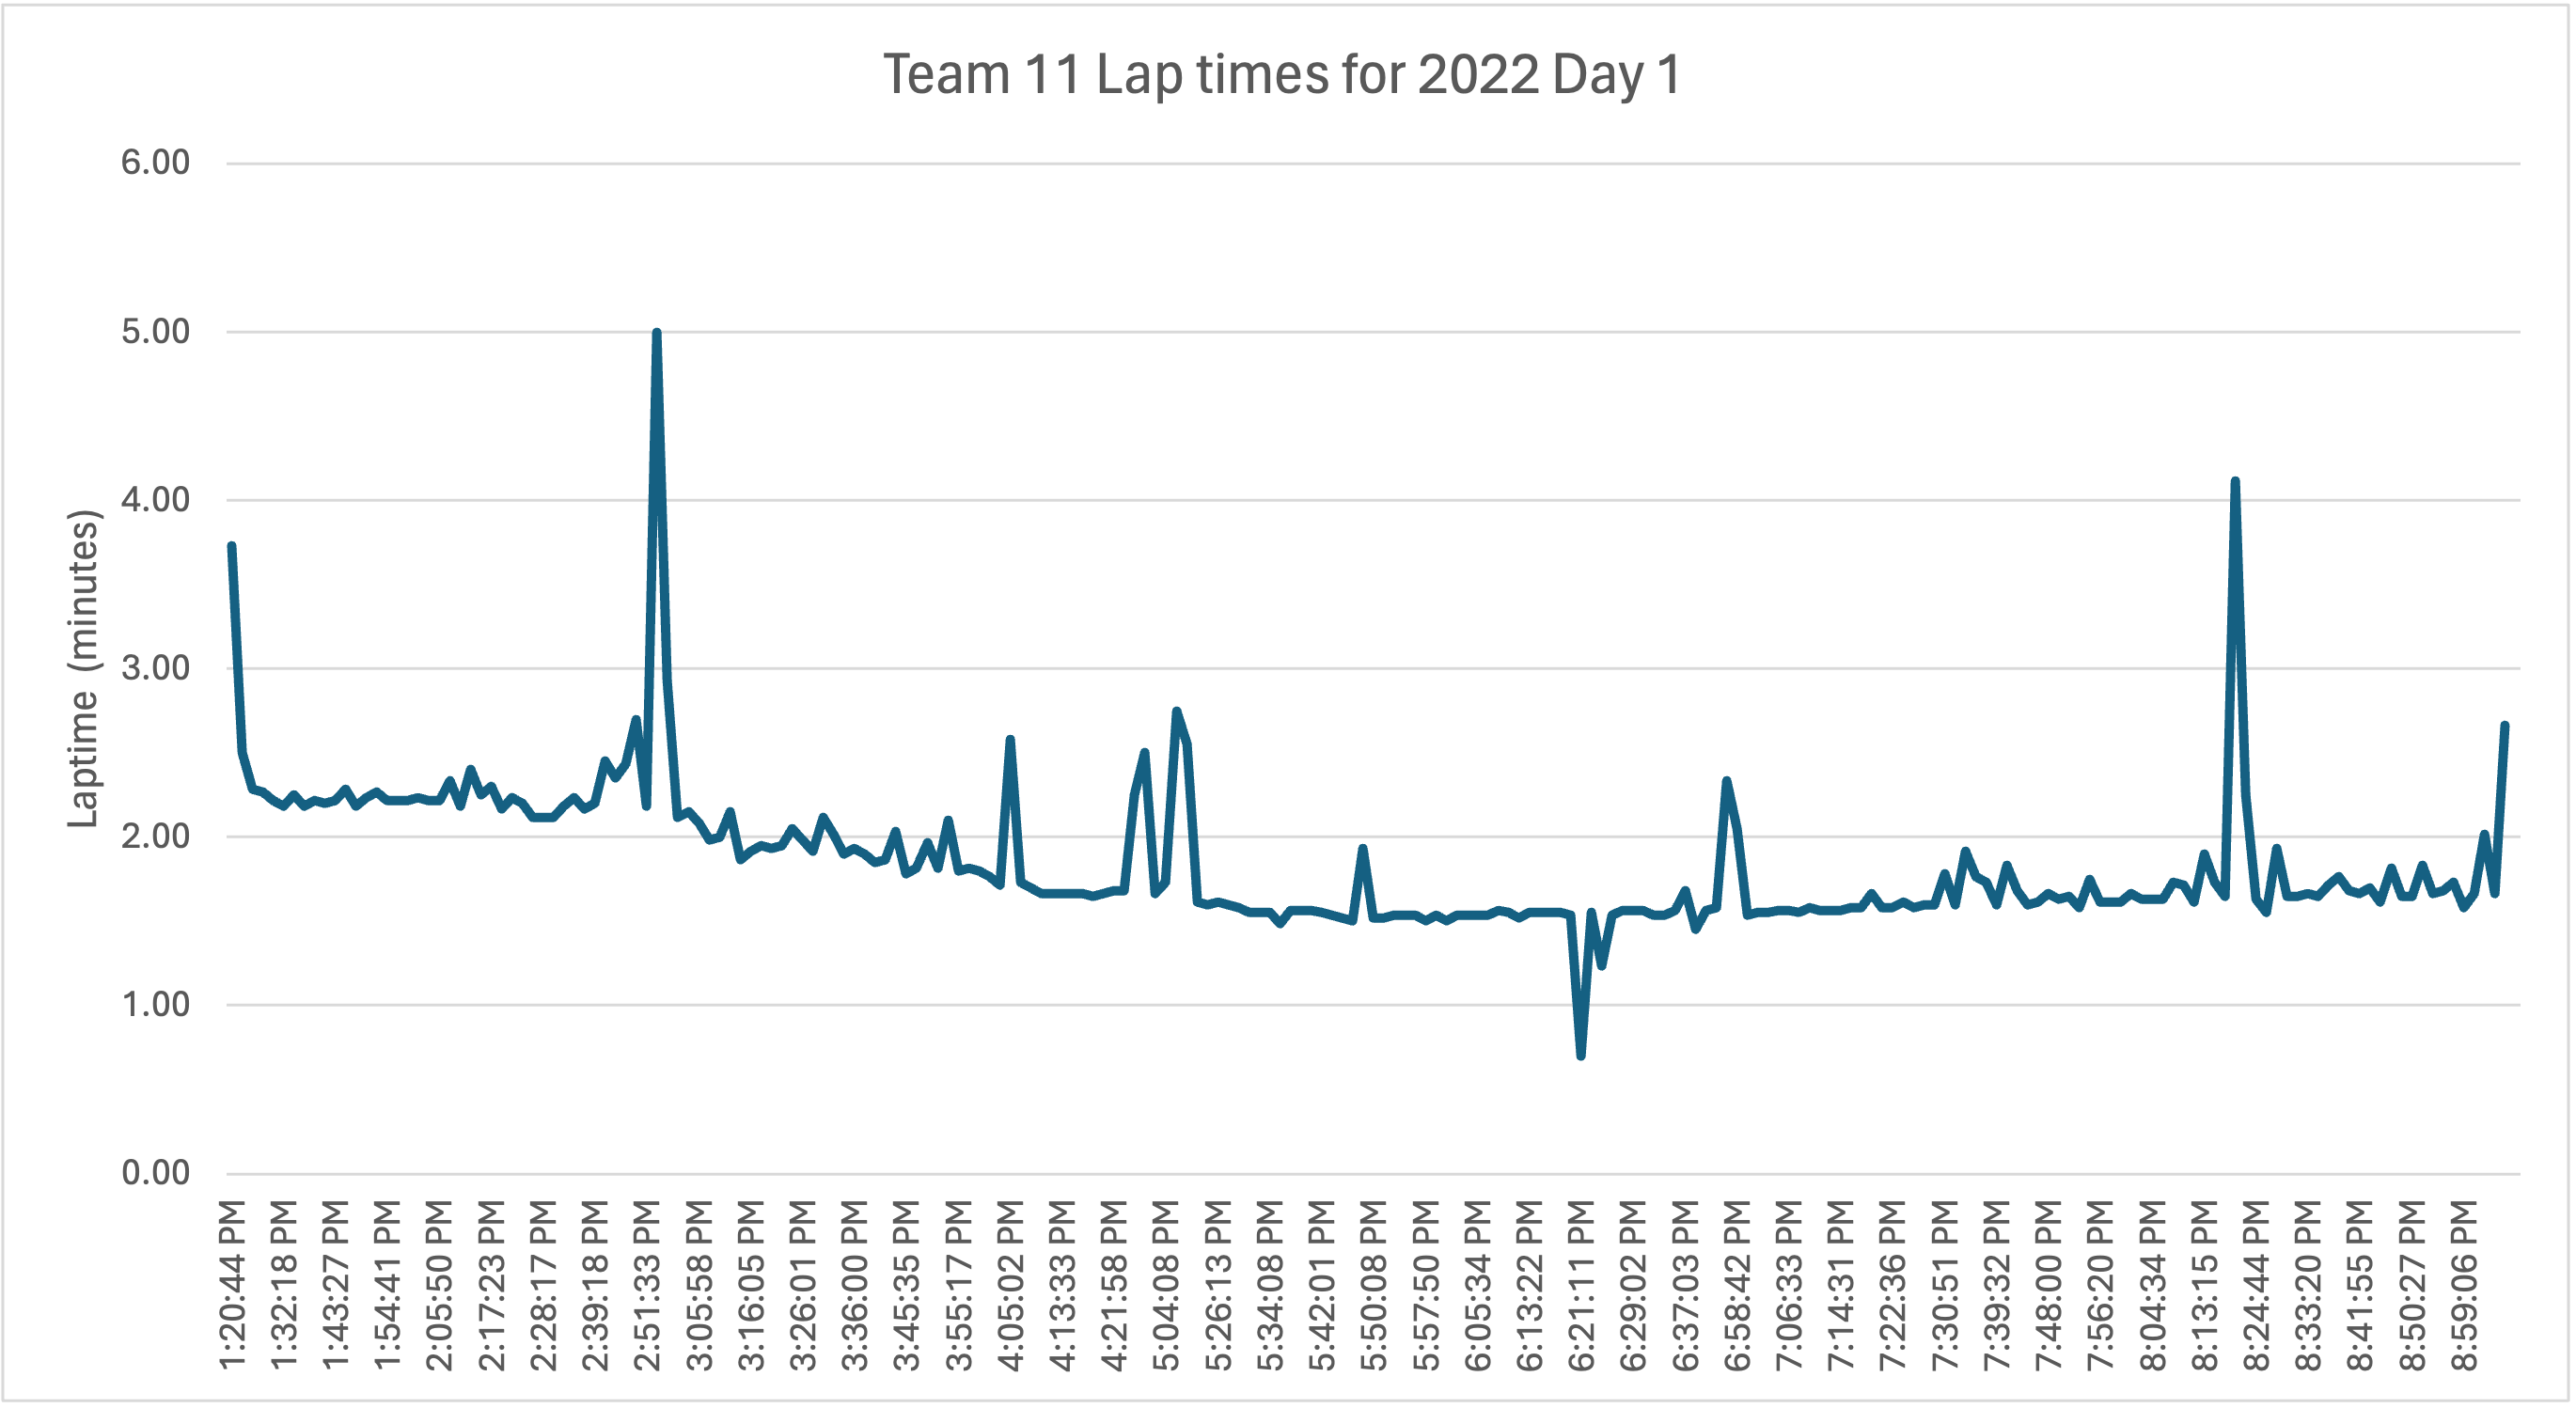
\includegraphics[width=0.8\textwidth]{team11_lap_times.png}
    \caption{Lap Times for Team 11}
    \label{fig:team_11_lap_times}
\end{figure}


\pagebreak
\subsection{Judge Accuracy Query}

A key metric which is useful in selecting which judges are allowed to continue their role in scoring is the accuracy of their scoring. This query calculates the accuracy of each judge by determining the number of "bad events" recorded by each judge. Bad events are determined based on certain criteria:

\begin{itemize}
    \item The time of the event is more than one standard deviation away from the average time of all records for the same team and time interval (lap).
    \item The time range of the events for the same team and time interval is greater than one second.
\end{itemize}

\noindent
The query outputs the following fields:

\begin{itemize}
    \item \textbf{judge\_name:} Name of the judge.
    \item \textbf{bad\_events:} Count of bad events recorded by the judge.
    \item \textbf{total\_events:} Total count of events recorded by the judge.
    \item \textbf{bad\_event\_rate:} Rate of bad events recorded by the judge.
\end{itemize}

\begin{lstlisting}[style=sql, caption={Query to calculate timing stats}, label={lst:sql_judge_accuracy_query}, ]
-- Calculate the count of "bad events" for each judge
-- Bad events are determined based on certain criteria
WITH judge_counts
        AS (SELECT subquery.judge_name,
                    COUNT(*) AS bad_events
            FROM (
                    -- Subquery to compute metrics and filter bad events
                    SELECT lr.*,
                            grp.avg_event_count,
                            TO_TIMESTAMP(grp.avg_time)      AS avg_time,
                            grp.std_dev_timestamp,
                            EXTRACT(
                                EPOCH
                                FROM
                                TO_TIMESTAMP(grp.max_time) -
                                TO_TIMESTAMP(grp.min_time)) AS time_range,
                            CASE
                            WHEN
                                grp.std_dev_timestamp !=
                                0
                                THEN
                                (EXTRACT(
                                    EPOCH
                                    FROM
                                    lr.time_stamp) -
                                grp.avg_time) /
                                grp.std_dev_timestamp
                            ELSE NULL
                            END                           AS num_std_devs,
                            REGEXP_REPLACE(
                                LOWER(SUBSTRING(
                                    lr.judge
                                    FROM
                                    POSITION(
                                        '-'
                                        IN
                                        lr.judge) +
                                    1)),
                                '\d',
                                '')                         AS judge_name
                    FROM score_rawclickeydata lr
                            JOIN (
                    -- Subquery to calculate aggregated metrics
                    SELECT team_id,
                            (EXTRACT(
                                EPOCH
                                FROM
                                time_stamp) /
                            30)::INT *
                            30               AS time_interval,
                            AVG(
                            COUNT(*))
                            OVER (PARTITION BY team_id,
                                (EXTRACT(
                                    EPOCH
                                    FROM
                                    time_stamp) /
                                30)::INT)     AS avg_event_count,
                            AVG(EXTRACT(
                                EPOCH
                                FROM
                                time_stamp)) AS avg_time,
                            STDDEV(EXTRACT(
                                EPOCH
                                FROM
                                time_stamp)) AS std_dev_timestamp,
                            MIN(EXTRACT(
                                EPOCH
                                FROM
                                time_stamp)) AS min_time,
                            MAX(EXTRACT(
                                EPOCH
                                FROM
                                time_stamp)) AS max_time
                    FROM score_rawclickeydata
                    GROUP BY team_id,
                                (EXTRACT(
                                    EPOCH
                                    FROM
                                    time_stamp) /
                                30)::INT) grp
                                ON lr.team_id =
                                    grp.team_id
                                AND
                                    (EXTRACT(
                                        EPOCH
                                        FROM
                                        lr.time_stamp) /
                                    30)::INT *
                                    30 =
                                    grp.time_interval
                    ORDER BY lr.team_id,
                            (EXTRACT(
                                EPOCH
                                FROM
                                lr.time_stamp) /
                            30)::INT *
                            30) AS subquery
            -- Filtering criteria for bad events
            WHERE ABS(subquery.num_std_devs) >
                    1
                AND subquery.time_range >
                    1
            GROUP BY subquery.judge_name),
-- Calculate the total count of events for each judge
        total_judge_counts
        AS (SELECT REGEXP_REPLACE(
                        LOWER(SUBSTRING(
                            raw_data.judge
                            FROM
                            POSITION(
                                '-'
                                IN
                                raw_data.judge) +
                            1)),
                        '\d',
                        '')  AS judge_name,
                    COUNT(*) AS total_events
            FROM score_rawclickeydata AS raw_data
            GROUP BY judge_name)
-- Join the counts of bad events and total events for each judge
-- Also calculate the bad event rate for each judge
SELECT judge_counts.judge_name,
        bad_events,
        total_events,
        CASE
            WHEN
                total_events !=
                0
            THEN
                CAST(bad_events AS FLOAT) /
                total_events
            ELSE 0
            END AS bad_event_rate
FROM judge_counts
        JOIN total_judge_counts
            ON judge_counts.judge_name =
                total_judge_counts.judge_name
-- Order the results by the count of bad events in descending order
ORDER BY bad_events DESC;
\end{lstlisting}

\begin{table}[H]
    \centering
    \caption{Sample query results from Listing \ref{lst:sql_judge_accuracy_query}.}
    \label{tab:my-table}
    \begin{tabular}{|c|c|c|c|}
        \hline
        \textbf{judge\_name} & \textbf{bad\_events} & \textbf{total\_events} & \textbf{bad\_event\_rate} \\ \hline
        Judge 1              & 429                  & 3510                   & 0.122                     \\
        Judge 2              & 153                  & 2666                   & 0.057                     \\
        Judge 3              & 110                  & 3818                   & 0.029                     \\
        Judge 4              & 90                   & 1238                   & 0.073                     \\
        Judge 5              & 81                   & 490                    & 0.165                     \\
        Judge 6              & 77                   & 1176                   & 0.065                     \\
        Judge 7              & 24                   & 679                    & 0.035                     \\
        Judge 8              & 12                   & 130                    & 0.092                     \\
        Judge 9              & 11                   & 279                    & 0.039                     \\
        Judge 10             & 11                   & 340                    & 0.032                     \\
        \hline
    \end{tabular}
\end{table}


While not explicitly what the query was designed for, an interesting observation made from one of the subqueries while developing the query was the distribution of consistency in the time intervals between events. As shown in Figure \ref{fig:time_interval_distribution}, the overall distribution of time intervals between events is quite uniform, with a peak around 0 seconds. This indicates that most events are recorded in quick succession, which is expected given the nature of the competition. This also shows that over 90\% of the events are recorded within 2 seconds of each other, which is a good sign of consistency in the data.

\begin{figure}[H]
    \centering
    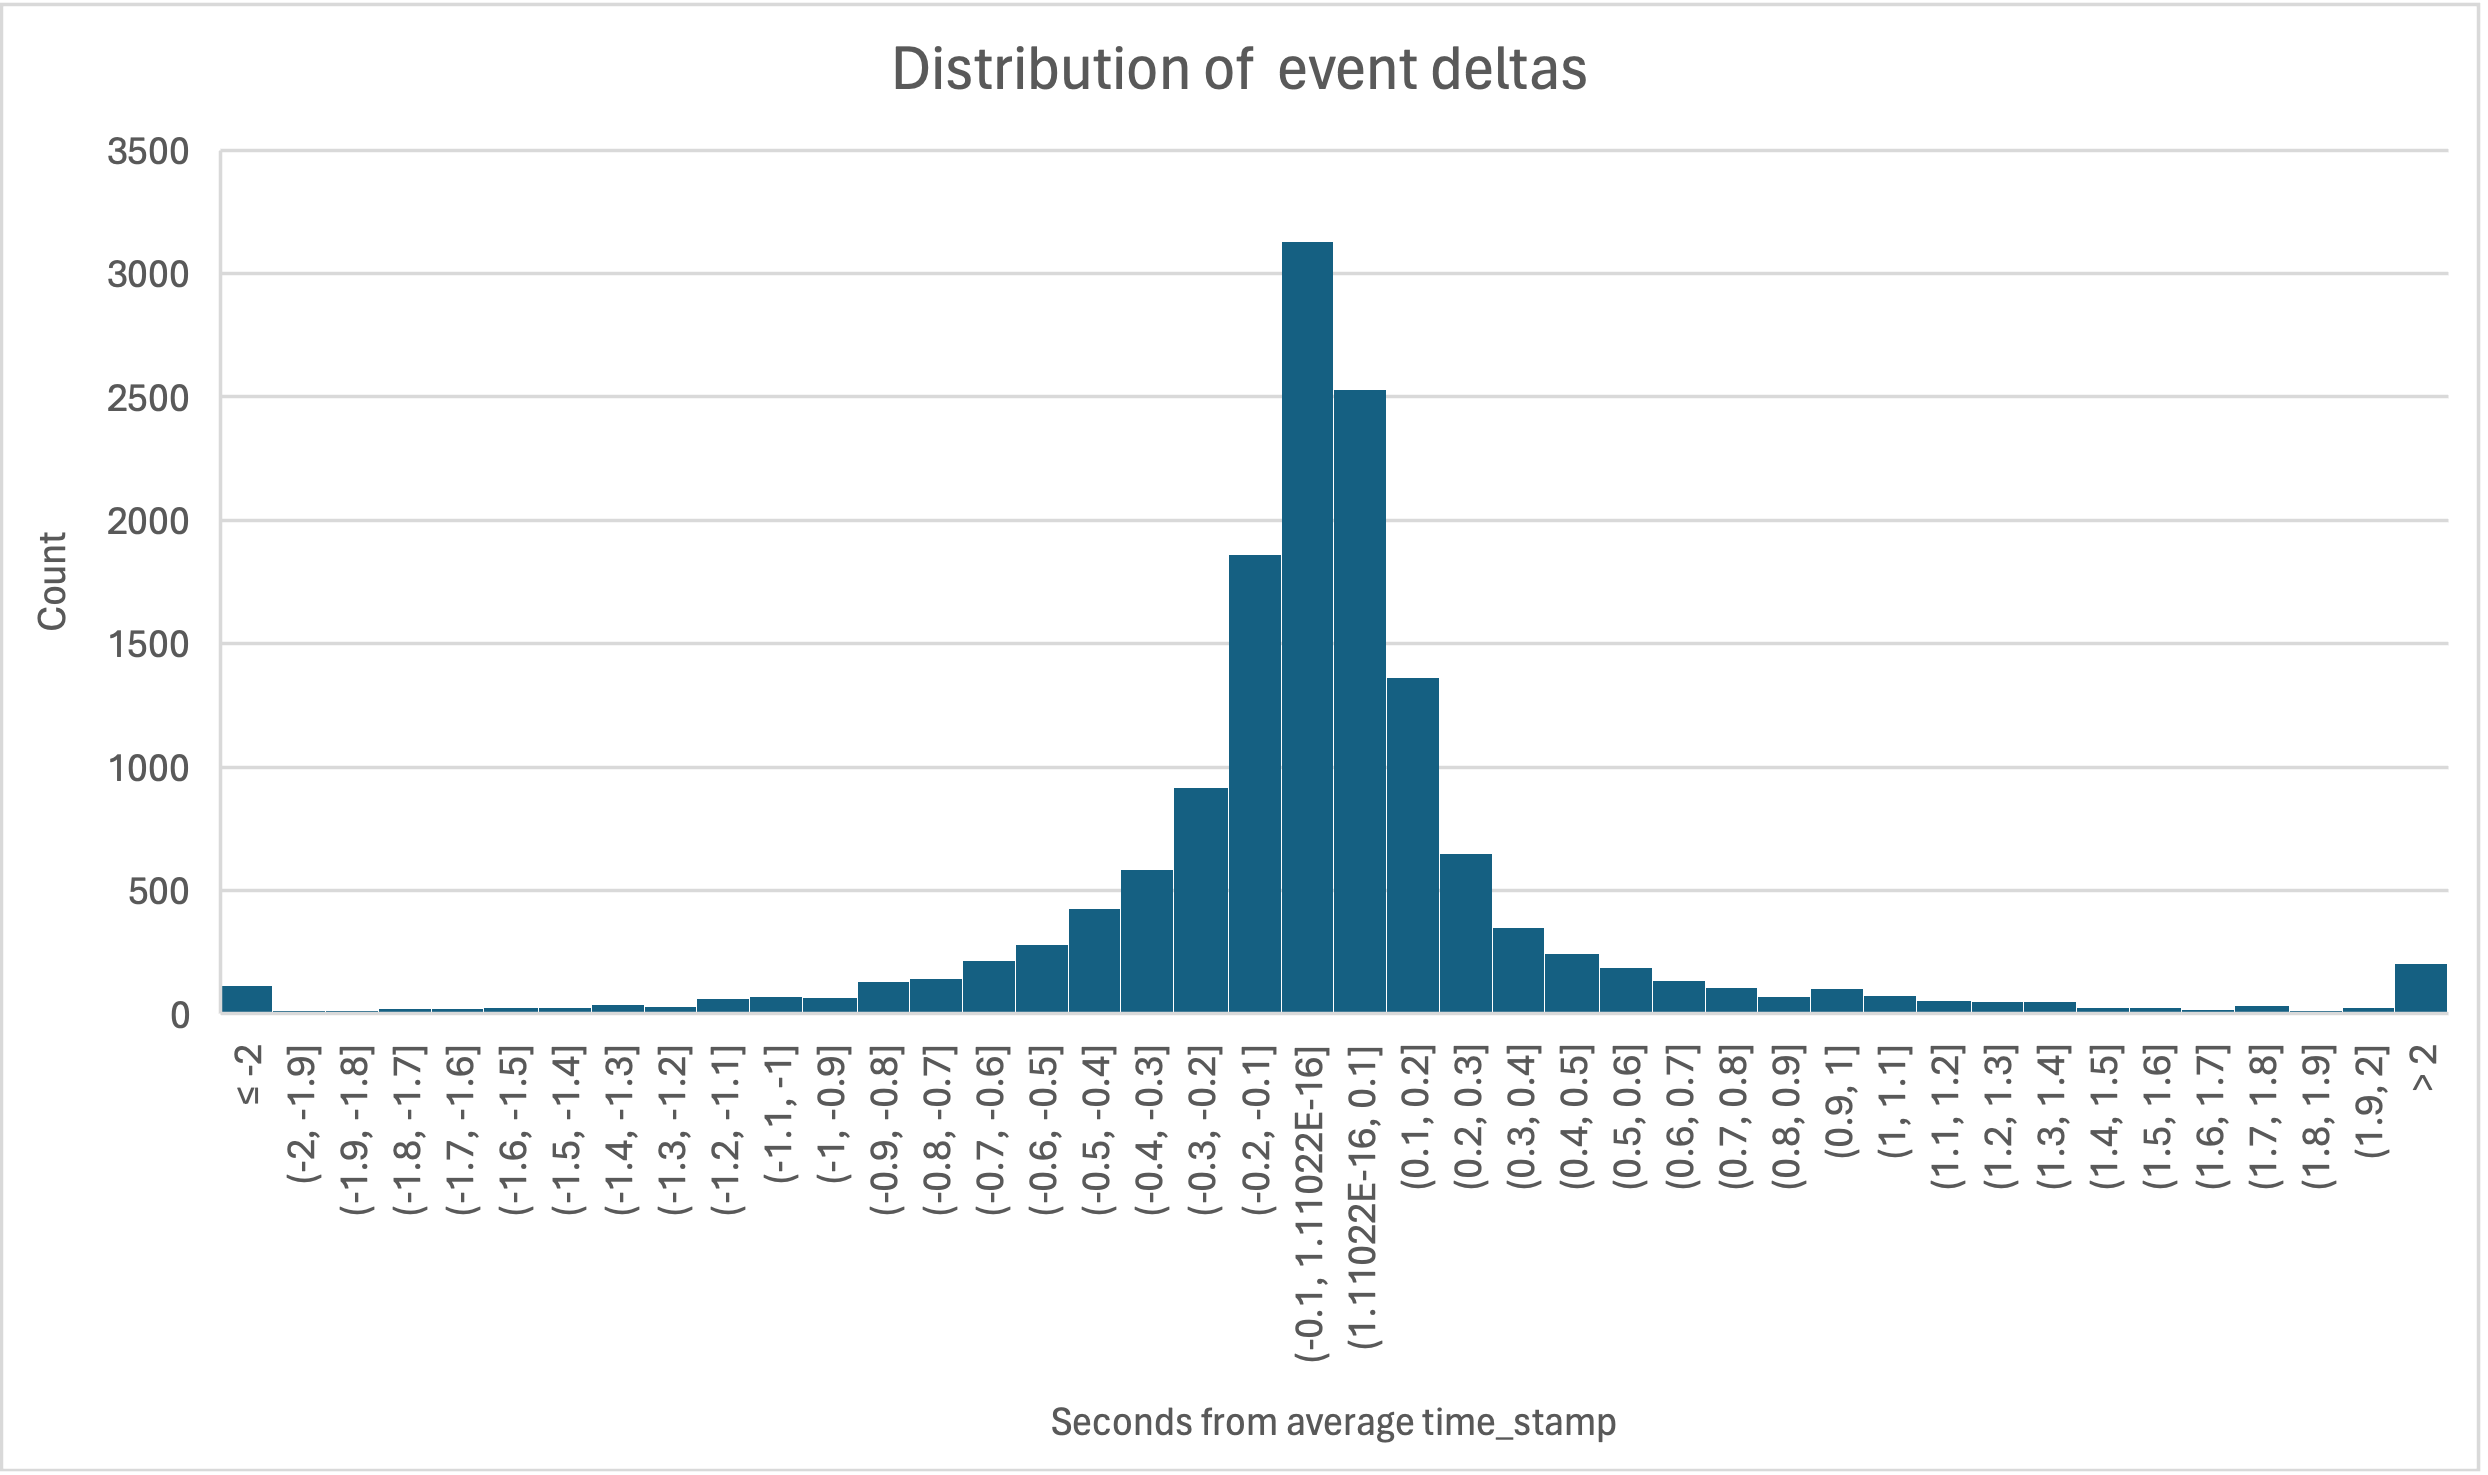
\includegraphics[width=0.8\textwidth]{distribution.png}
    \caption{Distribution of time intervals between events.}
    \label{fig:time_interval_distribution}
\end{figure}







\section{Technical Challenges}


The primary technical challenge encountered was a few missing tables from the archived dataset. Fortunately, these missing tables were not critical to the analysis and could be reconstructed from the available data. Reconstruction was conducted using publicly available information on the SCCF website, along with my knowledge of the event and some placeholder data.

Somewhat surprisingly, one of the biggest challenges was formatting the SQL queries to fit within the page margins for this report. Most of the queries were quite long and required significant effort to format correctly. Apologies for the weird formatting and somewhat hard to read queries.


\section{Tools Used}

The primary tool used in the analysis was PostgreSQL as the dataset was stored in a PostgreSQL database. Both VS Code and DataGrip were used in the writing of the queries, however all executions occurred in DataGrip as it provided the best UI for viewing the results. All graphs presented in this report were generated by exporting the results to CSV and imported into Excel for processing. The final report was written in LaTeX using VS Code (Because local development is superior! Sorry Overleaf).



\end{document}